\documentclass{standalone}
\usepackage{tikz}
\usetikzlibrary{arrows.meta, backgrounds}

\begin{document}
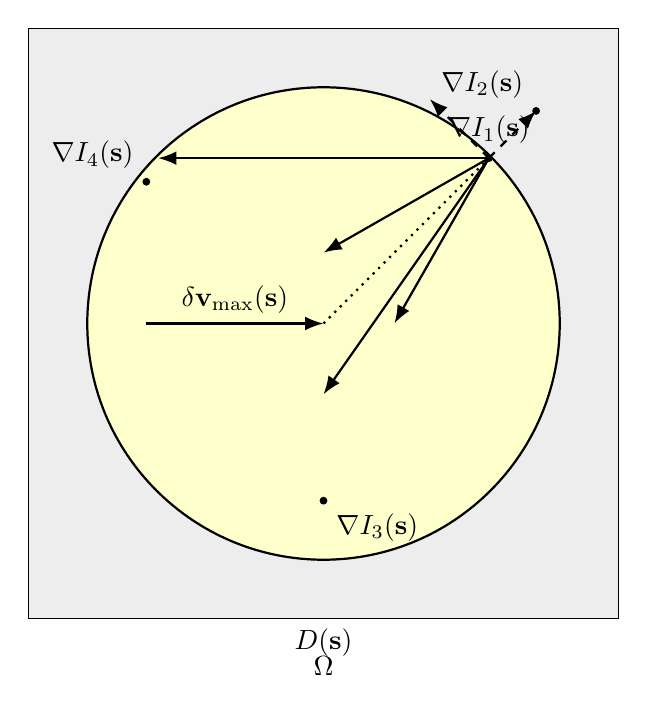
\begin{tikzpicture}[scale=1.5]

% Define colors
\definecolor{lightgray}{RGB}{220, 220, 220}
\definecolor{lightyellow}{RGB}{255, 255, 204}

% Background rectangle
\draw[fill=lightgray!50] (-2.5,-2.5) rectangle (2.5,2.5);

% Circle representing D(s)
\draw[fill=lightyellow, draw=black, thick] (0,0) circle (2cm);
\node at (0,-2.7) {$D(\mathbf{s})$};

% Labels for gradients
\node[circle, fill=black, inner sep=1pt, label={above:$\nabla I_1(\mathbf{s})$}] at (1.4,1.4) {};
\node[circle, fill=black, inner sep=1pt, label={above left:$\nabla I_2(\mathbf{s})$}] at (1.8,1.8) {};
\node[circle, fill=black, inner sep=1pt, label={below right:$\nabla I_3(\mathbf{s})$}] at (0,-1.5) {};
\node[circle, fill=black, inner sep=1pt, label={above left:$\nabla I_4(\mathbf{s})$}] at (-1.5,1.2) {};

% Arrows for gradients
\draw[-{Latex}, dashed, thick] (1.4,1.4) -- (1.8,1.8);
\draw[-{Latex}, dashed, thick] (1.4,1.4) -- (0.9,1.9);
\draw[-{Latex}, thick] (1.4,1.4) -- (0,0.6);
\draw[-{Latex}, thick] (1.4,1.4) -- (-1.4,1.4);
\draw[-{Latex}, thick] (1.4,1.4) -- (0.6,0);
\draw[-{Latex}, thick] (1.4,1.4) -- (0,-0.6);

% Delta vector
\draw[{Latex}-, thick] (0,0) -- (-1.5,0) node[midway, above] {$\delta\mathbf{v}_{\max}(\mathbf{s})$};
\draw[dotted, thick] (0,0) -- (1.4,1.4);

% Outer boundary label
\node at (0,-2.9) {$\Omega$};

\end{tikzpicture}
\end{document}